% !TEX root = _main.tex
% ========================================
% 卒業論文 本文
% ========================================
\section{はじめに}

2025年11月28日に和田山特別支援学校で開催されたUD交流会(「DXでつながるワトクの学び」)に参加した.

本報告書では,UD交流会に向けて制作した作品の内容と,交流会当日の様子および交流会の参加を通して得られた反応や知見について報告する.

本交流会に参加することになったきっかけは,同ゼミ生の存在である.
同ゼミ生が障がい者支援の分野に関心を持っており,その関係から本交流会の開催を知った.
筆者自身も映像表現やエンターテインメント分野に興味があり,多くの人に楽しんでもらうためにはどのような表現や体験を制作すべきかを考えるよい機会になると考えた.
本交流会への参加経験が今後の筆者自身の研究活動につながると考え,参加を決意した.

今回は,壁面と床面と身体動作を組み合わせて,参加者の身体動作に応じて映像やエフェクトが変化する体験型展示を制作した.
特別な操作説明を必要とせず,児童生徒が直感的に楽しみながら体験できることを目標として制作を行った.

%2
\section{和田山特別支援学校UD交流会について}
UD交流会はユニバーサルデザインのゲームおよび,デジタルデータをもとに創造物を制作する技術であるデジタルファブリケーション
\cite{IB_Hyoguchi23}
,そして生成AIと多様なツールを活用し,児童生徒が地域と交流を深める可能性を探るものであり\cite{He26},
大きく3つの目的がある.

\begin{enumerate}
	\item ユニバーサルデザインのゲーム交流会を通じて,児童生徒が地域の方と協力しながら活動する中で,協調性やコミュニケーション能力を育む
	\item デジタルファブリケーション体験会を通じて,特別支援学校におけるデジタル技術を活用したモノづくりの可能性を広げ,創造的な学びのきっかけを提供する
	\item 生成AI活用研修会を通じて,教育現場でのAI活用の最新事例や実践的な活用方法を学び,特別支援教育における新たな実践アイデアの創出につなげる
\end{enumerate}

参加者は,特別支援学校の小学部から高等部までの児童生徒65名およびその保護者,
その他の県立の特別支援学校,朝来市・養父市の福祉及び行政関係者,
近隣の福祉介護施設の方,放課後等デイサービスの事業者の方である\cite{watoku}.



%3
\section{制作に向けて}


%3.2
\subsection{特別支援学校見学}
会場となる体育館の下見を兼ねて,和田山特別支援学校の見学を行った.
見学を通して筆者にとって特に印象に残った点は,学年のみでクラスを分けを行うのではなく,一人ひとりの障がいの程度に応じたクラス分けが行われていたことである.
また,掲示物による情報伝達においても,文字情報のみでは理解が難しい場合に対応し,文字と対応した画像を併記することで,情報が伝わりやすく工夫されていた.
さらに,最新の技術も積極的に取り入れることで,学校内にとどまらず地域とのつながりへと活動を広げている点も印象に残った.

%3.4
\subsection{制作の初期構想}

次に,制作の初期構想について記述する.体験に明確なルールを設けるゲーム性のあるものと,ルールを必要としない体験型表現の二つの方向性で検討を行った.  

ゲーム性があるものとして2つの案を出した.

1つ目は,体験する人がチャンバラ棒を持ち,それを振ると壁に映された自分のキャラが同じように動くものを制作し,
対戦形式の遊びやミッションを設け,対象物を攻撃してもらい時間内にどれだけのミッションを成功できるかというものである.

2つ目は,画面上に対象物が現れ,その対象物に触れることで消え,時間内にどれだけ多く消せるかを目指すゲームの制作である.

一方で,ゲーム性なしの方向では,床と壁それぞれの制作案を出した.

壁は,画面に巨大な楽器を映し出し,楽器を弾くときに実際に押さえるところを光で教え,その光の部分に触れることでその楽器の音が鳴り,エフェクトが出現するものである.

床は,水面など実際にその場を歩いているような体験ができるものを考えた.

同ゼミ生などと話し合いをし,最終的に
壁に触れることで楽器の切り替えと楽器の音を鳴らし,エフェクトが出現するという体験ができるものと,
床にもプロジェクターで投影させ,実際にその場を歩いているような体験ができ,音を拾いその音に合わせてオブジェクトが増えていくものに決定した.

最終的にゲーム性を持たない体験型表現を採用した理由としては,ゲーム性を持たせる場合にはルール説明が必要となり,参加者の年代の幅も広いことから,
ルールの理解が少し困難になる可能性があると考えた.

そこで,触れるという直感的な操作によって音が鳴り,演出や床の表現が変化する
体験であれば複雑な説明が必要なく手軽に楽しめるのではないかと考えた.

%4
\section{制作}

先ほど記述した最終案に基づき,実際に制作した作品について記述する.

今回制作した作品は,MediaPipeを使用して参加者の身体座標を取得し,その動きに応じて映像や音,エフェクトが変化する展示である.

展示は大きく「壁」と「床」の二つの要素で構成されている.
壁面では,ボタンに触れることで演奏される楽器が切り替わり,表示された楽器に触れると対応した音が鳴り,視覚的なエフェクトが出現する仕組みとなっている.

一方,床面では,図1のような歩いた位置に応じてエフェクトが出現する演出に加え,参加者の動きに合わせて動物が追従する表現や,壁側で発生した音に反応して床にエフェクトが現れる演出を制作した.

壁面の展示については制作の途中までは制作を担当し,その後同ゼミ生へ引き継ぎを行った.
今回の報告書では,床面の展示の制作について詳しく説明する.

\begin{figure}[t]
	\centering
	\includegraphics[width=\linewidth]{3h.png}
	% ファイルパスに注意、0.8は一度小さくして、合わせてる?\linewidthはそのまま?
	\caption{システム図}\label{fig:animator}
\end{figure}

%4.1
\subsection{展示構造}
\figref{fig:system}のようにプロジェクターを上から床に向けて投影し,カメラをプロジェクターの左側に設置した.
カメラも対象者の全身,画面の全体が映る様にプロジェクター同様上から撮影を行った.
この設置構成は、MediaPipeで肩まで検出する必要があったためである.

\begin{figure}[t]
	\centering
	\includegraphics[width=\linewidth]{3a.png}
	% ファイルパスに注意、0.8は一度小さくして、合わせてる?\linewidthはそのまま?
	\caption{設置図}\label{fig:system}
\end{figure}

%4.2
\subsection{MediaPipeとは}

MediaPipeとは画像や動画からモーションキャプチャーのように骨格検出を行うことができるGoogleが開発したオープンソースのライブラリであり,
手先の位置から各関節位置を検出することが可能である\cite{Yuki513024}.

最大の特徴は,ネットワーク通信においてデータが送信元から受信先まで直接伝送される高速なエンドツーエンド処理\cite{EndToEnd}を可能にし,リアルタイム性を必要とするアプリケーションに対応できる点であり,多くのプラットフォームでも利用可能で,開発者にとって非常に柔軟なツールになっている.
今後も,エンターテインメント,医療,教育など様々な分野での応用が期待されている\cite{Isso2024}.

\subsubsection*{(1)MediaPipeの利点}

\begin{itemize}
	\item 高速な処理能力と汎用性
	\item エンドツーエンドの設計:特定のタスクを効率的に実行でき,従来の手法に比べて大幅な処理時間の短縮につながる
	\item カスタマイズ性に優れ,独自のユースケースに応じた調整が可能
\end{itemize}

\subsubsection*{(2)基本構成と役割}

データ入力,モデル推論,データ変換,結果出力という一連のプロセスを包括的に管理するモジュールで構成されている.

主な機能としては以下のものなどが挙げられる

\begin{itemize}
	\item 顔認識
	\item 手の検出
	\item 姿勢推定
	\item 物体検出
\end{itemize}

%4.2.1
\subsection{制作におけるMediaPipeの役割}
今回の制作において,MediaPipeを用いた足位置検出や座標変換を行うプログラムは同ゼミ生が実装し,筆者はコードを受け取りUnity側での制作を行った.

今回のMediaPipeのコードは,
カメラ映像から取得した人の足の位置を検出,足の動きを「左/右/停止」で判定し,実際の床上の座標(0~1の正規化座標)に変換し,その位置と移動方向をUnityにUDP通信によってリアルタイムに送信することを目的としている.
具体的なコードの動きとしては以下のようになっていた.

まず,床座標への変換を行うために,別プログラムを用いてカメラ映像上の床の4隅を指定する.

この時,画面上で左上→右上→右下→左下の順にクリックし,最大4点までの位置情報を記録する.
ここで記録された4点は「変換元座標」として,カメラ画像上における床の位置を表している.
一方,変換先座標として床全体を左上(0.0, 0.0),右上(1.0, 0.0),右下(1.0, 1.0),左下(0.0, 1.0)とする正規化された2次元空間の定義を行っている.
この変換元座標と変換先座標を対応付けることで,射影変換(ホモグラフィ)行列の計算を行う.これにより,カメラの角度や遠近によって歪んだ床領域を,正規化された正方形の座標空間へ変換することが可能である.
計算されたホモグラフィ行列がファイルとして保存され,後述する足位置検出のプログラムで読み込んで使用するものである.

足位置検出プログラムでは,使用するカメラ番号と足が「動いた」と判定するための最小移動量(閾値)を設定している.今回の制作では微妙な小さい揺れを無視するため,移動量の閾値を0.005に設定した.
プログラムを開始するとカメラが起動し,MediaPipePoseが初期化される.これにより,映像内の人の骨格情報が推定され,左右それぞれの足先が取得される.
MediaPipeで取得される座標は0~1の正規化座標であるため,画面幅および高さを掛けることで画像座標に変換している.
取得した足先位置は,左足が緑色,右足が赤色の円としてPCの画面上に表示し,正しく検出できているかを視覚的に確認できるようにしている.

次に,事前に作成したホモグラフィ行列を使って,画面座標から床座標(0~1)への変換を行う.これにより,カメラの設置位置や角度に依存しない,床上での正規化された足位置を取得できる.

足の移動方向は,前フレームの足位置と現在の足位置との差分を計算することで判定している.
x方向の変化量が閾値を超えた場合にのみ,左方向または右方向への移動として認識し,小さな動きは無視される.

最終的に,左右それぞれの足について,移動方向および床座標上の位置情報をJSON形式にまとめ,UDP通信を使用しローカル環境上のUnityへリアルタイム送信している.
Unity側では,この情報をもとにエフェクトの生成や演出制御を行っている.

%4.3
\subsection{MediaPipe(Python)からUnityへ送信}
先ほど記述したMediaPipeのコードによって取得された足の位置情報及び移動方向をUnity側の演出に反映させるため,本制作ではPython側で算出されたデータをUnityへ送信し,それを受信・処理するプログラムを実装した.
Python側で取得した人の動きや位置情報は,UDP通信を用いてUnityにリアルタイムで送信され,その情報をもとにUnity内で演出制御が行われる.
この構成によって,Unity単体では処理負荷が大きくなりやすいカメラ映像の解析や人の位置・足・手の検出,動きの方向判定などの処理をPython側に分離することが可能になっている.

Python側では,まずはカメラ映像・センサー入力をもとに人の体の位置や動きの方向を解析し,左右それぞれの足の位置を床全体を0から1の範囲で表した正規化座標として算出する.
同時に,足の移動量から移動方向を判定し,その結果を文字列データとして保持する.
これらの位置情報及び移動方向はJSON形式にまとめられ,UDP通信を使用してローカル環境上のUnityへ送信される.

Unity側では,このJSONデータを受信するためのスクリプトとしてPythonReceiverを実装している.
プログラム開始時にUDP通信を開始し,指定したポート番号を使用してPythonから送信されるデータの受信を待機する.
UDP通信処理はUnityのメインスレッドとは別スレッド上で実行されており,常に最新のデータを取得することが可能である.この構成により,人の動きに対して遅延の少ないリアルタイムな反応が実現されている.


受信したデータはJSONとして解析され,左右それぞれの移動方向情報および足位置の正規化座標がUnity内の変数として保持される.
これにより,Python側で計算された結果をUnity内の他のスクリプトから参照し,演出制御に利用することが可能となる.

取得された足位置の座標は0から1の範囲で正規化された値であるため,Unityのワールド空間内で直接使用することができない.
そこでUnity側では,床として設定していたPlaneオブジェクトを基準とし,正規化座標をワールド座標へ変換する処理を行っている.
この変換では,Planeの大きさおよび位置を考慮し,正規化座標の中心をPlaneの中央に対応させることで,カメラ映像上で検出された人の位置とUnity内の床上の位置とを対応付けている.

この座標変換処理を利用することで,人が実際に立っている位置や踏み込んだ位置に応じて,床上にエフェクトやオブジェクトを出現させるといった演出が可能になる.
また,今回のプログラムでは左右それぞれの移動方向も同時に取得しているため,動きの「向き」や「状態」を演出に反映させることができる.
具体的には,動いているときエフェクトを発生させたり,移動方向に応じて映像やエフェクトの流れを変化させたりするなど,身体動作と連動した表現が実現されている.

以上のように,今回のプログラムはPython側からUDP通信によって送信されるJSONデータを受信し,左右の移動方向および位置情報をUnity内で扱える形に変換する役割を担っている.


%4.4
\subsection{床の制作}
先ほど記述した初期構想に基づき,床面を用いた体験型の演出を制作した.
当初は設定を水辺とし,参加者が実際にその場を歩いているような感覚を得られるものを目指し制作を行った.
具体的には,歩いた位置に波紋が広がる演出,水辺の動物が参加者の動きに合わせて追従する演出,
さらに,壁側で発生した音に反応して魚が増え,画面の中が次第に豊かになっていく構成を想定していた.

制作初期段階では,\figref{fig:process}のようにTouchDesignerで制作を行った.しかし,歩いた位置に応じて波紋を出すことが想定以上に困難であった.そのため,Unityを使用した制作に変更を行った.

\begin{figure}[t]
	\centering
	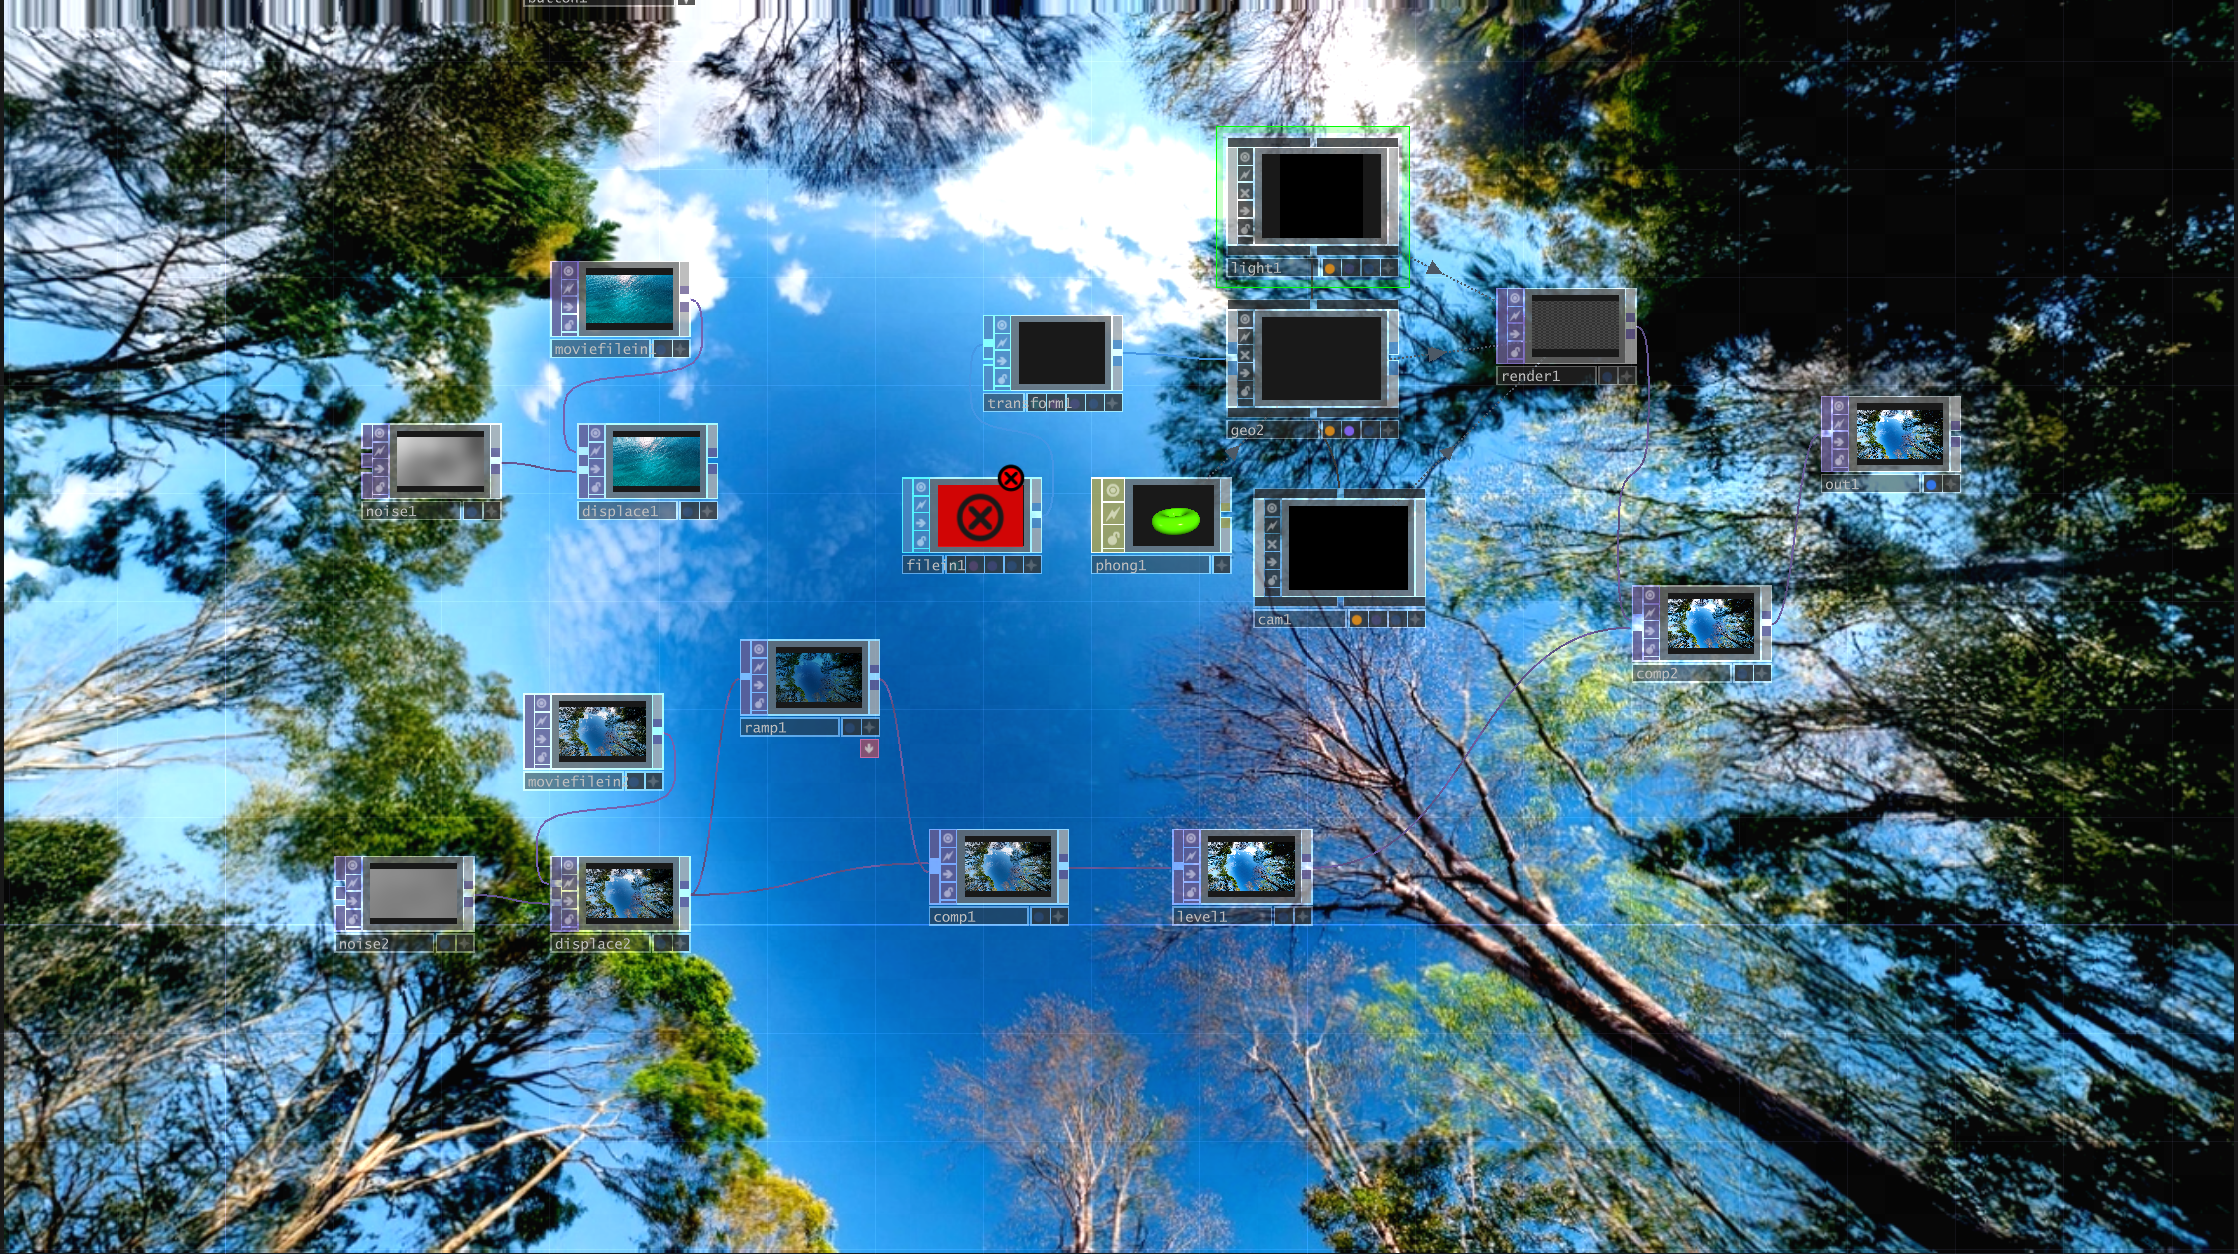
\includegraphics[width=\linewidth]{3b.png}
	% ファイルパスに注意、0.8は一度小さくして、合わせてる?\linewidthはそのまま?
	\caption{TouchDesignerでの制作過程}\label{fig:process}
\end{figure}


その後,制作を進める中で,出展予定の他の作品の中に,水面を使い「歩くことで変化する」演出を行う展示があることを知った.内容の重複を避けるため,歩くと変化するという制作内容はそのままにし,設定を水辺から\figref{fig:starry}のような星空へ変更することとした.
星空に変更した理由としては,映像表現ならではの非現実的な世界観にすることで,より楽しめる展示ができるのではないかと考えたためである.
加えて,壁側の展示がクリスマスの仕様に変更されていたことから,全体の雰囲気を合わせる狙いもあった.


\begin{figure}[t]
	\centering
	\includegraphics[width=\linewidth]{3c.png}
	% ファイルパスに注意、0.8は一度小さくして、合わせてる?\linewidthはそのまま?
	\caption{最終的に採用した床面の星空背景}\label{fig:starry}
\end{figure}



%4.4.1
\subsubsection{歩いた位置にエフェクト}
床を歩くと星が足元にエフェクトが散らばる表現を実現するために,Pythonで取得した左右の足位置情報をUnity側で受信し,それをもとにエフェクトを生成するものを制作した.
今回のシステムでは,左足および右足それぞれの位置情報を使用し,
前回エフェクトを生成した位置から一定以上移動していること,かつエフェクト生成のクールタイムが経過していることの両方を満たしている場合のみ,その位置に足跡エフェクトを生成する.

Pythonから受信される足位置座標は,Unity上で処理され,エフェクト生成の最短間隔は0.25秒に設定している.
これにより,1秒間に最大4回までエフェクトが生成されるよう制御している.
また,足が「動いた」と判定するために,前回の足位置からの移動距離が0.05以上であることを条件としている.

左右それぞれの足について,前回エフェクトを生成したときの位置情報を保持し,現在位置との差分から移動量を計算している.
同時に,前回の生成からどれだけ時間が経過したかを示すタイマーを左右独立で管理し,毎フレーム前フレームからの経過時間を加算することで時間計測を行っている.

エフェクト生成の判定処理では,前回位置から十分移動していることと,クールタイムが経過していることの両条件を満たす必要がある.
このクールタイムは,一度エフェクトを生成した後,次に生成可能となるまでの待ち時間であり,足が停止している場合にはエフェクトが生成されず,動いている場合でも過剰に生成されないように制御する役割を持っている.

条件を満たした場合,Python側の床座標系で表現された足位置をUnityのワールド座標に変換し,その位置に\figref{fig:effect}のようにエフェクトを生成する.
生成後は,現在の足の位置を「前回位置」として更新し,タイマーをリセットすることで次回の判定に備える構造となっている.

\begin{figure}[t]
	\centering
	\includegraphics[width=\linewidth]{3d.png}
	% ファイルパスに注意、0.8は一度小さくして、合わせてる?\linewidthはそのまま?
	\caption{歩いた位置にエフェクトが出現している様子}\label{fig:effect}
\end{figure}


%4.4.2
\subsubsection{トナカイの追従}
次に,人が歩くとその後を動物が追従してくる表現の制作について記述する.

今回のシステムでは,Pythonから送信される人の足の位置情報を使用し,Unity上で
トナカイの位置・向きとアニメーションを制御するコードを作成した.

まず,先ほど記述したPython側のMediaPipeから左右の足の位置情報を取得する.
この左右の足位置の平均をとることで,人の立ち位置を表す代表点を算出した.得られた情報はこれまでと同様,正規化された座標であるため,
Unityの空間上で扱えるようにワールド座標への変換を行っている.

次に,人とトナカイとの距離感を調整するため,追従距離をパラメータとして設定した.
追従距離の値を小さくする程,トナカイは人の近くに止まるようになる.
今回はUnity上で0.05の値を基準とし,床のスケールに応じて実際の距離が自然になる様に設定している.
また,トナカイの移動速度についてもパラメータ化を行い,Unity上で100の値を設定した.

アニメーションの制御には\figref{fig:animator}のようなUnityのAnimatorコンポーネントを使用した.
Animatorでは,「歩行(Walk)」や「着座(Sit)」のアニメーション状態を用意し,\verb|isSitting|というブール型パラメータを使用し状態遷移を制御している.
スクリプトのAnimatorコンポーネントを取得し,その後はスクリプトからこのパラメータを切り替えることでアニメーションを制御している.

\begin{figure}[t]
	\centering
	\includegraphics[width=\linewidth]{3e.png}
	% ファイルパスに注意、0.8は一度小さくして、合わせてる?\linewidthはそのまま?
	\caption{Animatorコンポーネント}\label{fig:animator}
\end{figure}


動物の移動処理では,人のワールド座標位置とトナカイの位置との差分を計算することで,トナカイが人の位置へ向かうための方向ベクトルを求める.
また,トナカイが常に人の方向に向くように回転処理を行っているが,y座標(高さ)を固定することで,首だけが左右に動くような自然な追従表現を実現している.

さらに,人との距離を一定に保つため,人の位置そのものではなく,そこから一定距離手前を目標位置として設定している.
これにより,トナカイが人に重なってしまうことを防ぎ,適切な距離感を保った追従が可能となっている.

最後に,トナカイと人との距離を毎フレーム確認し,距離が一定以下になった場合には着座アニメーションへ遷移させる.
一方で,距離が一定以上になると歩行アニメーションへと切り替える.このように距離条件に基づいてアニメーションを制御することで,
人が動けばトナカイが歩いて追従し,近づくとその場で座るという一連の自然な行動表現を実現した.

%4.4.3
\subsubsection{音に反応してエフェクト}
壁面から入力される音に反応し,床面上にエフェクトが発生するものを制作した.
今回のシステムでは,PCの内蔵マイクから取得した音声入力を用い,音の周波数成分に応じて異なるエフェクトを生成する.

今回使用したコードは,マイク入力の音をリアルタイムに周波数解析し,特定の周波数成分が一定の条件を満たした場合に,対応するエフェクトPrefabを上方向から生成するものである.
これにより,音の種類に応じて異なる視覚表現を床面に表すことが可能となっている.

まず,エフェクトPrefabの設定として二種類の音を判定対象とした.1つ目はA音とし,この音が検出された場合には雪のエフェクトが生成される.
2つ目はB音とし,この音が検出された場合には2種類の画像Prefabが同時に生成されるように設定した.
これにより,音の違いによって発生する演出を明確に切り替えるものを制作した.

音の検出条件としては,各音に対して閾値の設定および周波数を設定した.
A音およびB音の閾値はいずれも0.001とした.また周波数については,A音を440Hz,B音を2343Hzと設定した.

また,音が連続して入力された場合にエフェクトが過剰に生成されることを防ぐため,生成クールダウンを設定した.
今回は,同一エフェクトが連続して生成されない時間を0.5秒とし,前回エフェクトを生成した時刻と現在時刻を比較することで制御を行っている.

音声の入力にはPCの内蔵のマイクを使用し,取得した音は,時間領域の信号を周波数領域の情報に変換するFFT(高速フーリエ変換)\cite{Hy2125}によって周波数解析を行った.
FFTにより,入力された音は低音から高音までの周波数成分に分解され,それぞれの周波数帯における音の強さが配列として取得される.
この処理により,時間的な音の波形ではなく,周波数ごとのエネルギー分布として音を扱うことが可能となる.

A音の判定処理では,まず検出したい周波数が,解析された全周波数範囲の中でどの位置に相当するかを計算し,その結果をスペクトラム配列のインデックスとして求めている.
周波数に対応する配列番号が決定された後,その位置に格納されている値を取り出すことで,指定した周波数成分の音の強さを取得する.
取得した音の強さが,あらかじめ設定した閾値を超えており,かつ前回のエフェクト生成から一定時間が経過している場合にのみ,雪のエフェクトを生成する.

B音の判定処理についても,音の解析方法および判定の流れはA音の場合と同一である.
異なる点は,使用する周波数および閾値,そして生成されるエフェクトの内容である.
B音が条件を満たした場合には,二種類の画像Prefabが同時に生成されることでA音とは異なる視覚的演出が床面上に発生する.
\figref{fig:snow}は実際にエフェクトが降っている様子である.

以上のように,本システムでは音声入力を周波数成分として解析し,その結果に基づいてエフェクトを制御することで,音と視覚表現が連動した表現を実現している.


\begin{figure}[t]
	\centering
	\includegraphics[width=\linewidth]{3f.png}
	% ファイルパスに注意、0.8は一度小さくして、合わせてる?\linewidthはそのまま?
	\caption{エフェクトが降っている様子}\label{fig:snow}
\end{figure}


%5
\section{UD交流会に参加して}

今回のUD交流会に参加し,制作した作品に対して多くの好意的な反応を得ることができた.
実際に体験・見学していた児童や来場者からは「すごい」「かわいい」といったような意見をいただき,作品を楽しんでもらえている様子が見られた.
特に,床に投影された追従するトナカイの演出では,追従の動きを見るだけではなく,撫でたり踏んだりするなど
一人ひとり違う関わり方で楽しんでいる様子が印象的であった.
体験者自身が自由に関わり方を見つけて遊んでおり,今後の作品制作への解釈や考え方が広がるとても良い機会となった.

\begin{figure}[t]
	\centering
	\includegraphics[width=\linewidth]{3i.png}
	% ファイルパスに注意、0.8は一度小さくして、合わせてる?\linewidthはそのまま?
	\caption{実際に触れあっている様子}\label{fig:animator}
\end{figure}

以下では,今回の交流会への参加を通して得られたよかった点と課題点について,コミュニケーション面と制作面の2つの観点から記述する.

%5.1
\subsection{コミュニケーション面}
コミュニケーション面においては,どのようにすべきか迷っている生徒に対して,近くに歩み寄り,動き方や動くことによってどのような演出になるのかを説明することができた点が良かったと考える.
また,来場者から演出の仕組みやコードに関する質問された際にも,しっかり回答することができた.
さらに,床の方のみを体験して別のブースに行かれる来場者に対して壁側の体験展示に誘導できた場面もあり,作品全体を体験してもらうことができた点がよかったと考える.  

一方で課題点として,保護者からの質問には対応できていたものの,その後に生徒本人へ積極的に話しかけることが十分にできなかった点が挙げられる.
特に低学年の児童に多かったのが,視線が作品に向かない場面が多くみられた.床の演出は足元を見ることで変化が分かるものであったため,前を見たり,周囲を見回したりしているときに,この床の体験の意図が伝わっていなかったと考えられる.
その際,保護者が児童に対して説明している様子を見るだけになってしまい,自身から視線誘導を行うことができなかった場面が多くあった点は反省点である.


%5.2
\subsection{制作面}

制作面においては,大きなトラブルが発生することはなく,全体としては想定していた基本的な動作を実現することができた.
床の演出や追従するトナカイの動き,音に反応するエフェクトなども途中で止まることなく動いていた点はよかったと考える.  

一方課題点として,先ほども挙げた視線誘導ができなかったことが挙げられる.
床を見ずに体験する児童も多く,言葉による説明だけでなく,踏んだ時に音が鳴るようにするなど,演出で視線を下に誘導するような工夫が必要であったと考えられる.

MediaPipeを使用した座標取得については,検出は安定して行えていたが,肩まで写す必要がある構成であったため,カメラの高さや設置位置に制約ができた.
その結果,背の高い児童や来場者は動ける範囲が制限され,十分に楽しめなかった可能性がある.
また,投影される画面の大きさにも限界があり,床の演出変化は動くことで楽しさが伝わるものであったが,それが実現できない場面も見られた.

トナカイの追従演出に関しては,座標が常に場所を取得しているため,わずかな移動でも動いた判定になり,停止状態(STOP)の判定が難しかった.
そのため,トナカイが完全に止まることが少なく,停止中でも少しずつ動いてしまい変な挙動が発生することがあった.
また,車いすを利用している児童の場合,後ろを振り返ることが難しく,トナカイが追従していることが分かりにくくなってしまい,十分に楽しめなかった可能性がある.

音に反応するエフェクトについては,PCの内蔵マイクを使用して音を取得していたため,周囲の雑音にも反応していると考えられる場面が見られた.
また,エフェクトの出現が数秒間降り続ける演出であったことや,重なりすぎるのを避けるために出現間隔をあけていたことから,
音に反応していることが瞬時に分かりにくかったと考えられる.
一瞬でわかるようなエフェクトの出現方法や,音の種類ごとの差をより明確にする工夫が必要であった.

さらに,本番と同じ環境での十分なリハーサルが行えなかったことも課題として挙げられる.
カメラの位置調整や動作確認に想定以上の時間がかかり,うまくいかないことが多かった.

%6
\section{まとめ/今後の展望}
今回の報告書では,和田山特別支援学校で開催されたUD交流会に参加し,作品の制作および展示を行った内容について報告した.
今回の交流会を通して,来場者に楽しんでもらえた場面も多くあった一方で,必ずしもすべての参加者が十分に体験を理解し,楽しめていたとは限らないことも実感した.
実際に,制作した演出の意図や変化に気づかないまま他のブースへ移動する参加者や,システム上の限界により十分に体験できなかった参加者も見られた.
このことから,多くの人に楽しんでもらう作品を制作することの達成感と同時に,その難しさを感じた.

特に,体験者自身の動きによって変化しているということをどのように伝え,理解してもらうかという点は重要な課題であると考える.
人それぞれの性格や価値観,身体の使い方が異なる中で,体験の仕方も多様になるため,それらを考えて制作していく必要がある.
今回の制作で,映像などで非現実的な体験を実現できる表現の可能性を感じられ,体験の分かりやすさや参加者の多様性を意識した制作について考えられるいい機会となった.
今回の経験を踏まえ,今後はより多くの人に作品の意図が伝わり,楽しんでもらえるような制作に発展させたい.
